
%(BEGIN_QUESTION)
% Copyright 2006, Tony R. Kuphaldt, released under the Creative Commons Attribution License (v 1.0)
% This means you may do almost anything with this work of mine, so long as you give me proper credit

A solid metal cube measuring exactly 1 inch on a side is submerged in an open container filled with water.  The bottom of the cube is 24 inches down from the water's surface:

$$\includegraphics[width=15.5cm]{i00265x01.eps}$$

Based on your calculations of hydrostatic pressure (in PSI), determine the force applied to each side of the cube (in units of pounds), and the net, or {\it resultant} of these six forces (one force for each side of the cube).

Based on the figure for water density of 62.428 lb/ft$^{3}$, how much does one cubic inch of water happen to weigh?

\underbar{file i00265}
%(END_QUESTION)





%(BEGIN_ANSWER)

Force pushing up on cube's bottom face: 0.867 lb

Force pushing down on cube's top face: 0.831 lb

Average force pushing horizontally on each of the cube's four other faces: 0.849 lb

\vskip 10pt

Resultant force = 0.0361 lb (upward) = weight of 1 in$^{3}$ of water @ 62.428 lb/ft$^{3}$.

%(END_ANSWER)





%(BEGIN_NOTES)


%INDEX% Physics, static fluids: buoyancy

%(END_NOTES)


